\documentclass{article}
\usepackage{graphicx, amsmath}
\graphicspath{ {./images/} }

\title{Ch. 4.4 HW Solns}
\author{Mr. Spence}
\date{\today}

\begin{document}

\maketitle

\subsection*{QuickQuiz}

\begin{enumerate}
\setcounter{enumi}{9}

\item (b)
	\begin{figure}[h]
	\centering
	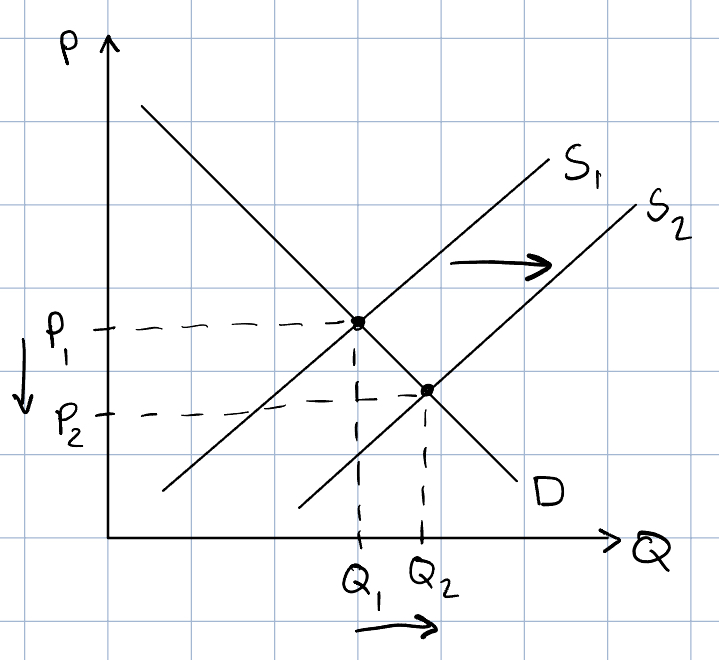
\includegraphics[width = 0.5\textwidth]{qq10}
	\end{figure}

\item (a)
	\begin{figure}[h]
	\centering
	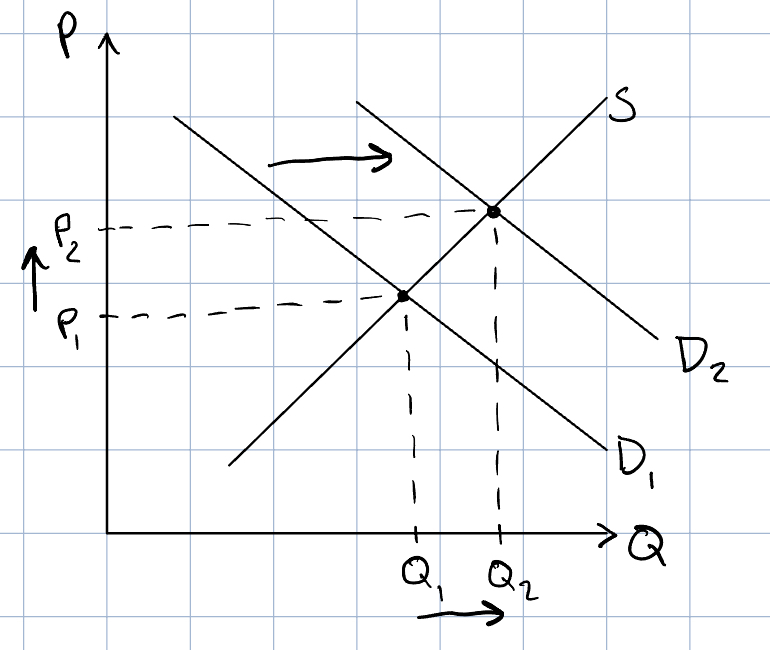
\includegraphics[width = 0.5\textwidth]{qq11}
	\end{figure}
	
\newpage

\item (c) -- For equilibrium price to increase and quantity to decrease, we need supply to shift left. That happens when input prices increase.
	\begin{figure}[h]
	\centering
	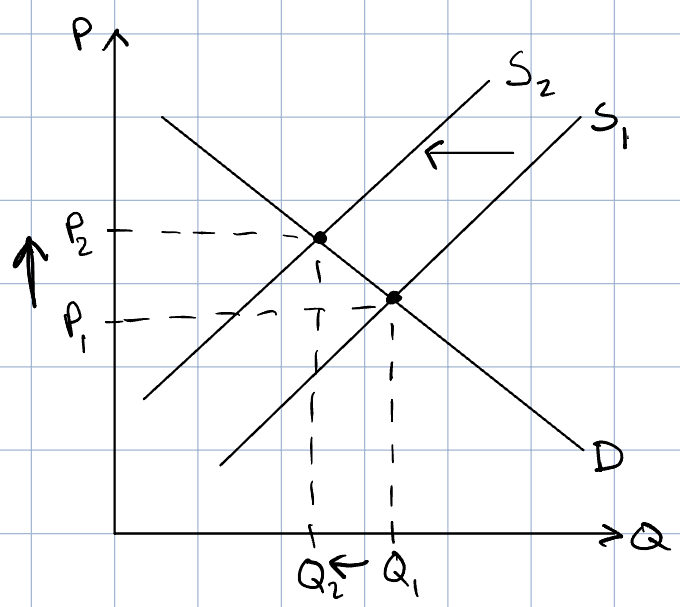
\includegraphics[width = 0.5\textwidth]{qq12}
	\end{figure}

\end{enumerate}

\subsection*{Problems and Applications}

\begin{enumerate}

\item
	\begin{enumerate}
	
	\item The cold snap will increase the cost of oranges, an input to OJ, because orange farms will be less productive. That shifts the supply of OJ to the left and increases the equilibrium price. 
	\begin{figure}[h]
	\centering
	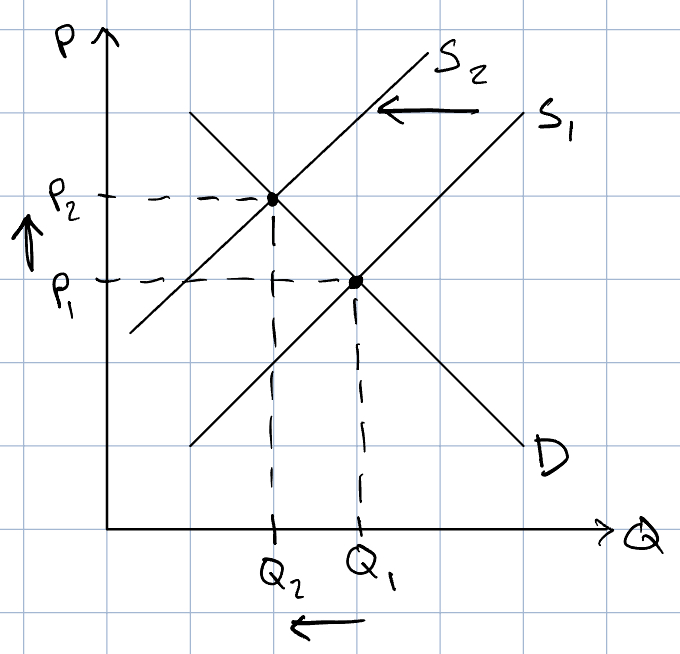
\includegraphics[width = 0.5\textwidth]{paa1a}
	\end{figure}
	
	\newpage
	
	\item People's preferences for hotel rooms move away from the Caribbean and towards New England. That decreases demand and drives down the equilibrium price.
	\begin{figure}[h]
	\centering
	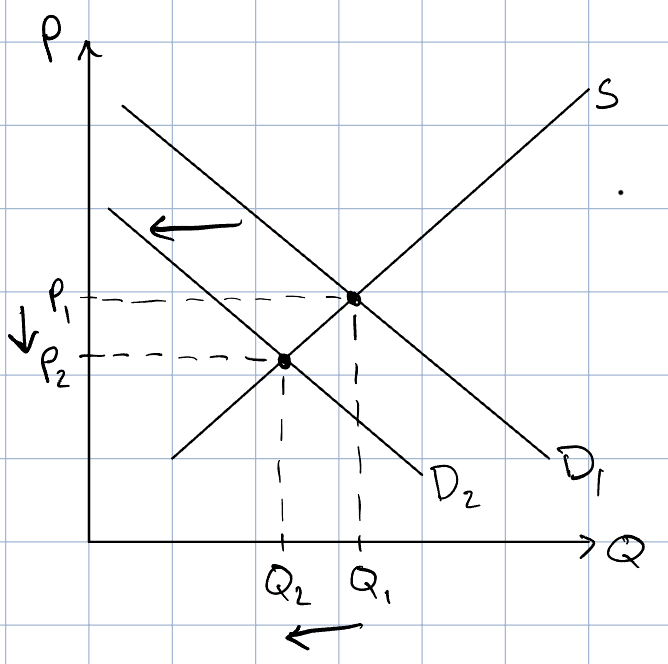
\includegraphics[width = 0.5\textwidth]{paa1b}
	\end{figure}
	
	\item When war breaks out in the middle east, the number of oil producers decreases. That shifts the supply of gasoline left which in turn increases the price of gasoline. Gasoline and cars are complements, so when the price of gasoline goes up, demand for cars shifts left and the price of cars drops.
	\begin{figure}[h]
	\centering
	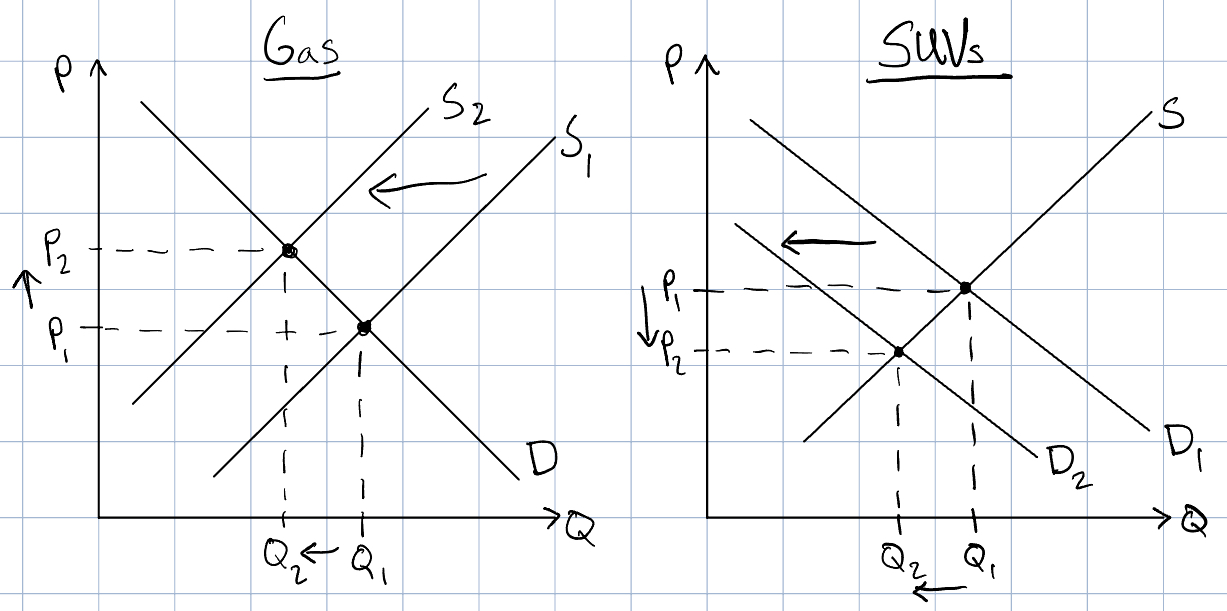
\includegraphics[width = 0.8\textwidth]{paa1c}
	\end{figure}
	
	\end{enumerate}
	
\newpage
	
\setcounter{enumi}{4}
\item Computer chips are an input for computers, so when the price of computer chips goes down, the supply of computers increases. As a result, price decreases and quantity increases in the market for computers.
	\begin{figure}[h]
	\centering
	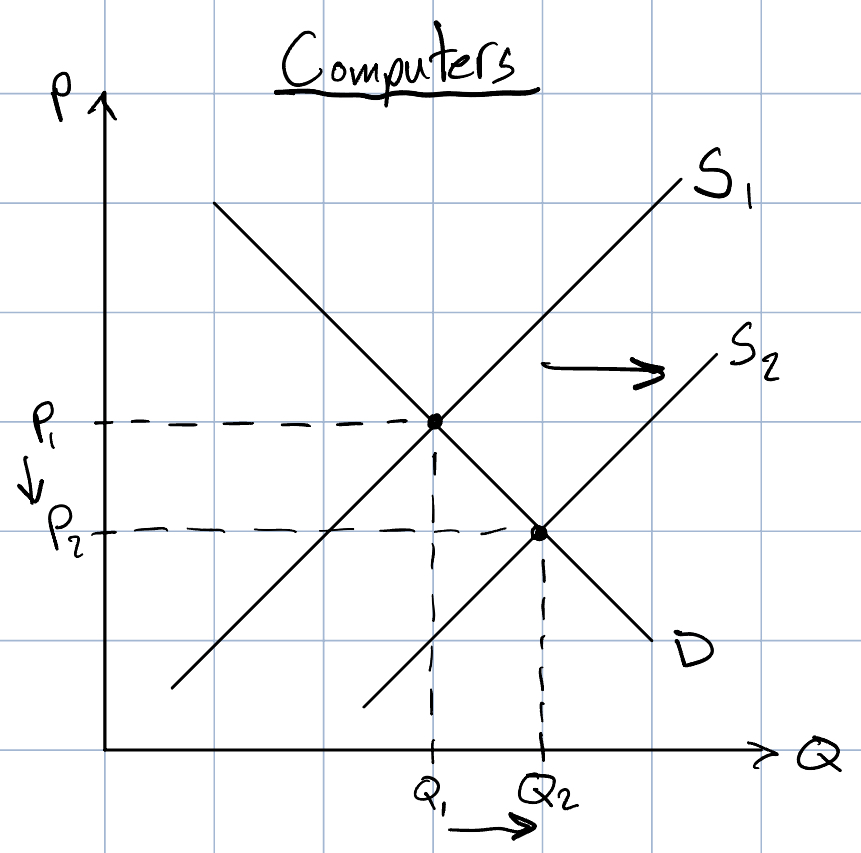
\includegraphics[width = 0.5\textwidth]{paa5_computers}
	\end{figure} 
	
	Computers and computer software are complements, so when the price of computers decreases, demand for computer software increases. That increases the price and quantity of computer software.
	\begin{figure}[h]
	\centering
	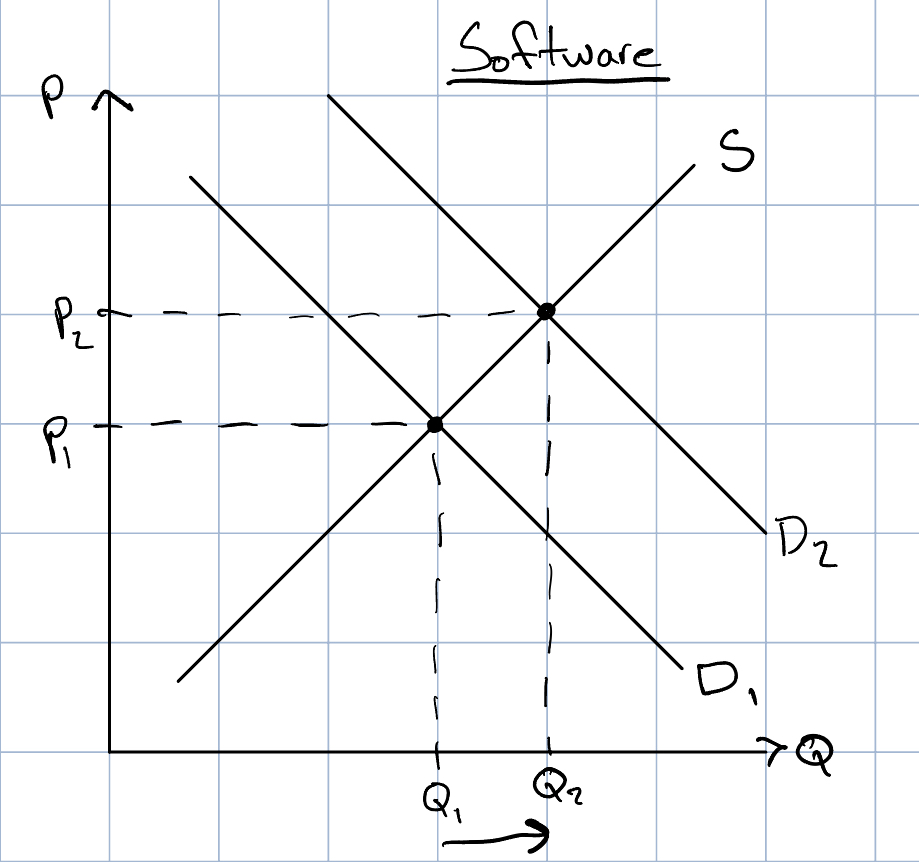
\includegraphics[width = 0.5\textwidth]{paa5_software}
	\end{figure}
	
	\newpage
	
	Computers and typewriters are substitutes, so when the price of computers decreases, demand for typewriters decreases. That decreases the price and quantity of typewriters. 
	\begin{figure}[h]
	\centering
	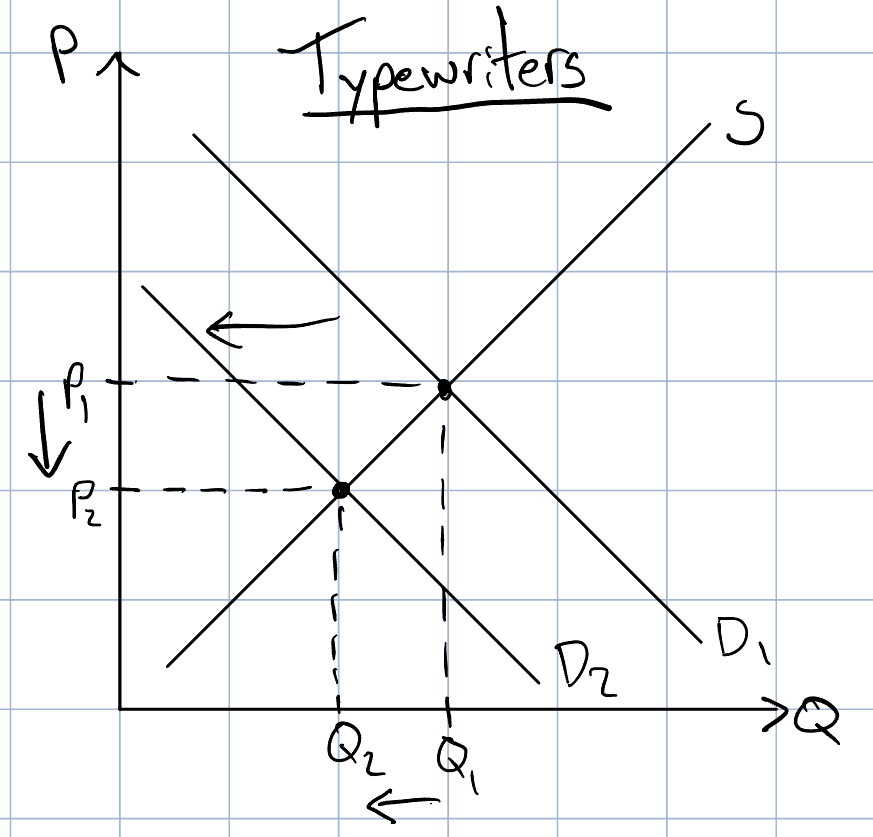
\includegraphics[width = 0.5\textwidth]{paa5_typewriters}
	\end{figure}
	
\item

	\begin{enumerate}
	
	\item The damaged crop will increase the price of cotton, so an input for sweatshirts becomes more expensive. That shifts supply left which increases equilibrium price and decreases equilibrium quantity.
	\begin{figure}[h]
	\centering
	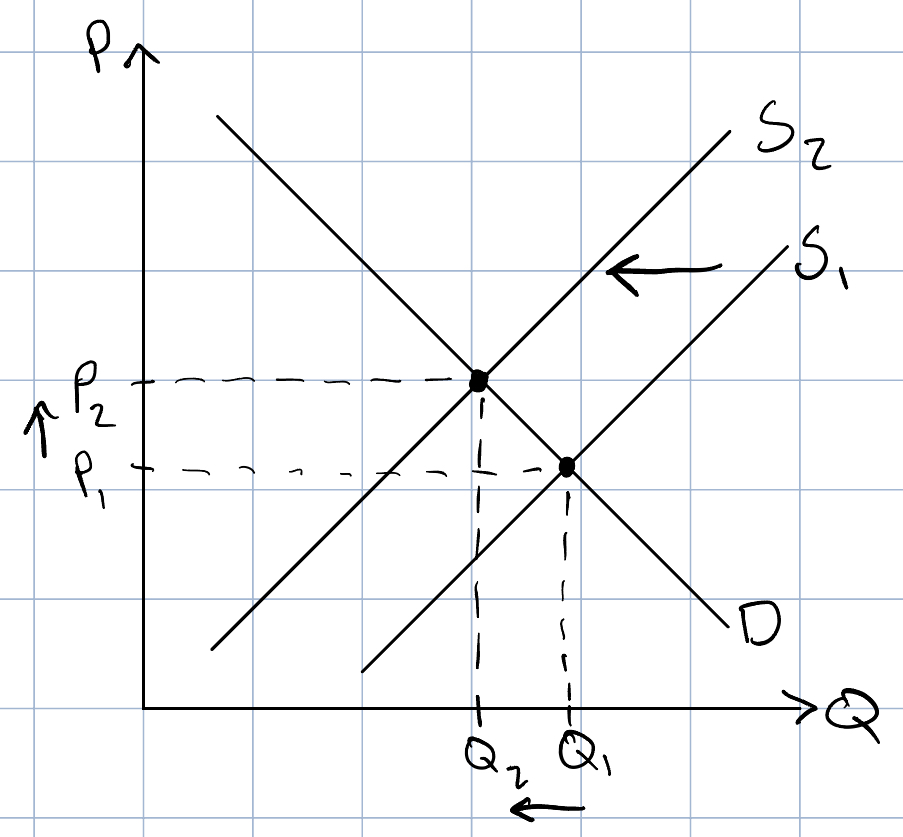
\includegraphics[width = 0.5\textwidth]{paa6a}
	\end{figure}
	
	\newpage
	
	\item The price of a substitute decreases, so demand shifts left. That decreases equilibrium price and quantity.
	\begin{figure}[h]
	\centering
	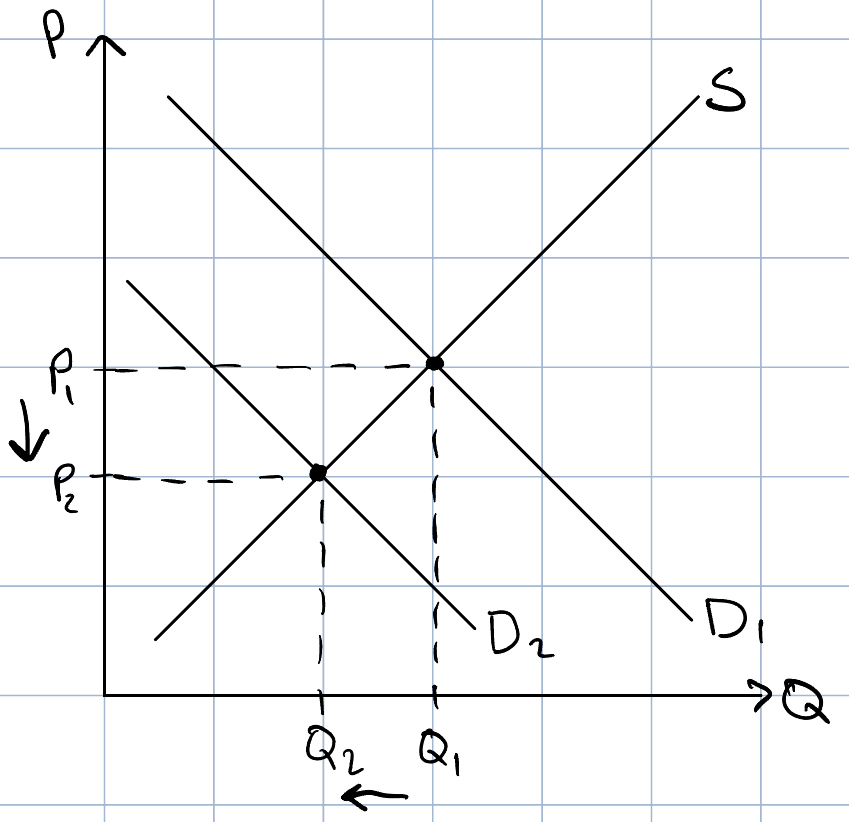
\includegraphics[width = 0.5\textwidth]{paa6b}
	\end{figure}
	
	\item The college mandate will increase the number of buyers which will shift demand right. That increases equilibrium quantity and price.
	\begin{figure}[h]
	\centering
	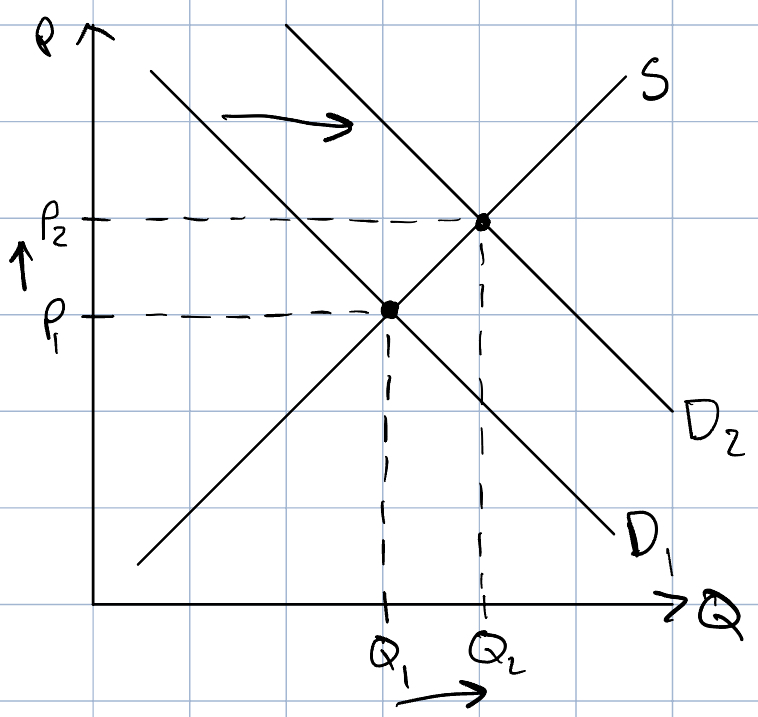
\includegraphics[width = 0.5\textwidth]{paa6c}
	\end{figure}
	
	\newpage
	
	\item The improvement in production technology will increase supply. That increases equilibrium quantity and decreases equilibrium price.
	\begin{figure}[h]
	\centering
	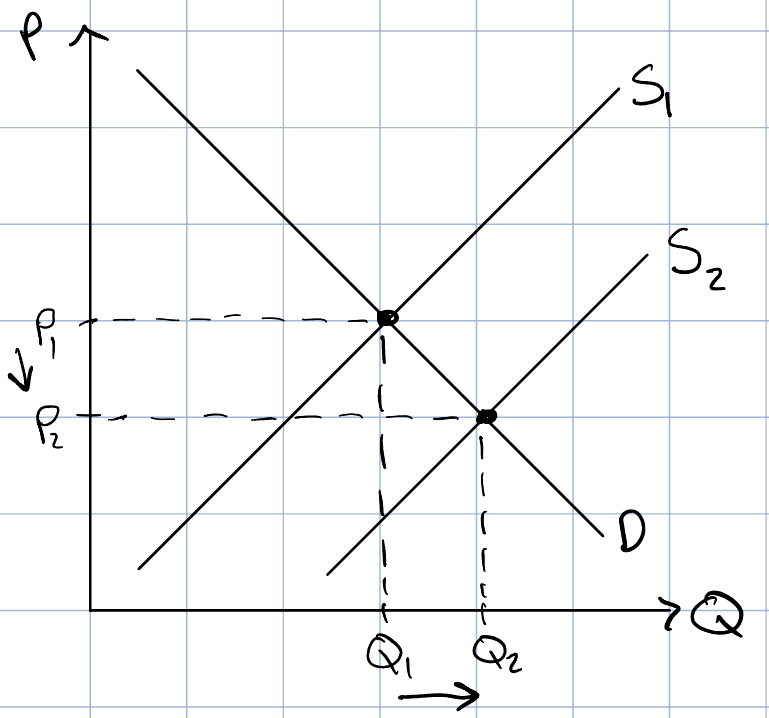
\includegraphics[width = 0.5\textwidth]{paa6d}
	\end{figure}
	
	\end{enumerate}

\setcounter{enumi}{7}	
\item 
	\begin{enumerate}
	
	\item The equilibrium price is \$6 because that's the price at which $Q_S = Q_D$. The equilibrium quantity is 81.
		\begin{figure}[h]
		\centering
		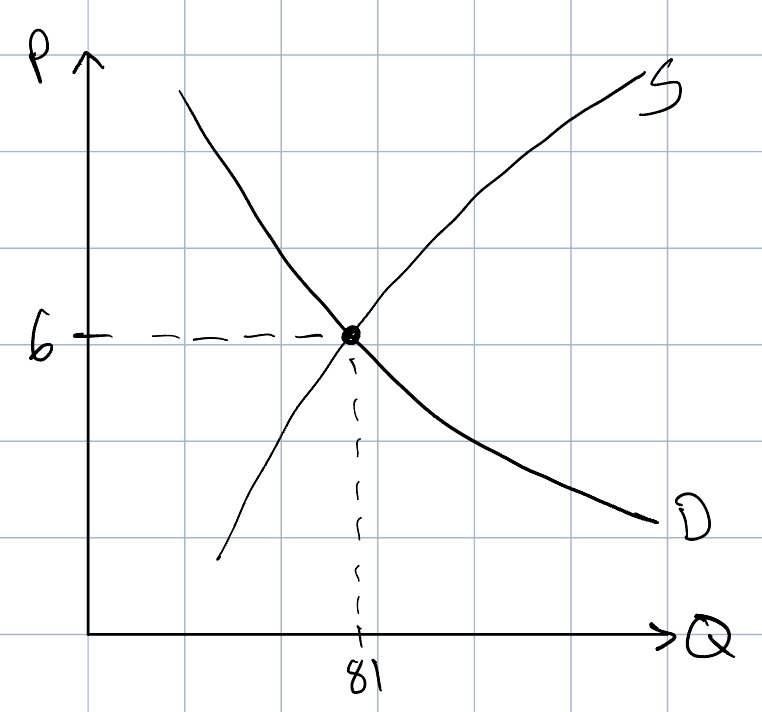
\includegraphics[width = 0.5\textwidth]{paa8a}
		\end{figure}
		
	\item There would be a surplus in which case $Q_S > Q_D$. That means not every seller would be able to find a buyer, so they would start cutting prices in an effort to attract them.
	
	\item There would be a shortage in which case $Q_S < Q_D$. That means not every buyer would be able to secure a pizza, so they start bidding up the price in an effort to secure one.
	
	\end{enumerate}

\end{enumerate}

\end{document}